% --------------------------------------------------------------
% This is all preamble stuff that you don't have to worry about.
% Head down to where it says "Start here"
% --------------------------------------------------------------

\documentclass[12pt]{article}

\usepackage[margin=1in]{geometry}
\usepackage{amsmath,amsthm,amssymb}
\usepackage{graphicx}
\usepackage{subcaption}
\usepackage{algorithmicx}
\usepackage{algorithm}
\usepackage{algpseudocode}
\usepackage[colorlinks,linkcolor=blue]{hyperref}
\usepackage[noabbrev]{cleveref}
\usepackage{courier}
\usepackage{listings}


\oddsidemargin 0in
\evensidemargin 0in
\textwidth 6.5in
\topmargin -0.5in
\textheight 9.0in

\newcommand{\ignore}[1]{}
\def\pp{\par\noindent}

\newcommand{\assignment}[4]{
\thispagestyle{plain}
\newpage
\setcounter{page}{1}
\noindent
\begin{center}
\framebox{ \vbox{ \hbox to 6.28in
{CIS 419/519: Applied Machine Learning \hfill #1}
\vspace{4mm}
\hbox to 6.28in
{\hspace{2.5in}\large\bf\mbox{Homework #2}}
\vspace{4mm}
\hbox to 6.28in
{{\it Handed Out: #3 \hfill Due: #4}}
}}
\end{center}
}

\makeatletter
\renewcommand{\fnum@algorithm}{\fname@algorithm}
\makeatother

\lstset{basicstyle=\footnotesize\ttfamily,breaklines=true}
\lstset{framextopmargin=50pt,frame=bottomline}


\begin{document}

\assignment{Fall 2024}{1}{September 11}{7:59 pm October 2}

% --------------------------------------------------------------
%                         Start here
% --------------------------------------------------------------


{\bf Name: }  Alan Wu\\

{\bf PennKey:} alanlwu\\

{\bf PennID:} 41855518

\section{Declaration}
\begin{itemize}
\item \textbf{Person(s) discussed with:} \textit{Peter Zhang, Arihant Tripathi}
\item \textbf{Affiliation to the course: student, TA, prof etc.} \textit{Students}
\item \textbf{Which question(s) in coding / written HW did you discuss?} \textbf{\textit{Question 1}}
\item \textbf{Briefly explain what was discussed.} \textit{Effect of scaling c on the capacity and bias and variance of model}
\end{itemize}

\section{Multiple Choice \& Written Questions}

\begin{enumerate}
\item 
\begin{enumerate}
\item Increase variance; bias stays the same
\item Decrease variance; Increase bias
\item Decrease variance; Increase bias 
\item Variance increases; Bias stays the same 
\item Variance stays the same; Bias stays the same 
\item for the following values to decrease test loss\\
    $n$: Increase n \\ 
    $\lambda$: Increase $\lambda$ \\ 
    $d$: Decrease $d$ \\ 
    $c$: Keep $c$ the same \\ 
    $\alpha$: Keep $\alpha$ the same 
\end{enumerate}

\item
\begin{enumerate}
\item To derive the gradient of the L1 regularization term for the: \\ 
We need to simply take the gradient of the equation with respect to $B_j$. 
\begin{align}
  L_{\ell_1} = \lambda \sum_{j=1}^{p} |B_j| \notag \\ 
  \frac{\partial L_{\ell_1}}{\partial B_j} = \lambda \text{ sign} (B_j) \notag
\end{align}

We ignore the case where $B_j = 0$ and derive that equation from the loss function. Notice that the gradient of the L1 regularized loss function
is only dependent on the sign of $B_j$ and the magnitude of $\lambda$.

\item  We can analyze the effect of the L1 regularization term on the parameters of the model by looking 
at the gradient of both the L1 regularization term and the MSE loss function with respect to $B_j$. \\ 

We can derive the full gradient of the loss function as such: 

\begin{align}
  L_{\ell_1} = \frac{1}{N} \sum_{i=1}^{N} (y_i - B^T x_i)^2 + \lambda \sum_{j=1}^{p} |B_j| \notag \\ 
  \frac{\partial L_{\ell_1}}{\partial B_j} = \frac{-2}{N} \sum_{i=1}^{N} (y_i - B^T x_i)x_{ij} + \lambda \text{ sign}(B_j) \notag
\end{align}

Part 1: The MSE Loss Term \\ 

We will discuss the two following cases: There is no dependency on the value of $\lambda$ in the MSE loss term.
\begin{enumerate}
  \item When $B_j$ is predictive of $y_i$ \\

  In this case, $B_j$ will be larger in magnitude and he gradient of the MSE loss term with respect to $B_j$ will be greater in magnitude. The gradient of the MSE loss term will also be larger, as it will influence changes in the gradient heavily.\\


  \item When $B_j$ is weakly or not predictive of $y_i$\\
  
  When $B_j$ is weakly or not predictive of $y_i$, $B_j$ will be smaller in magnitude (based on least squares regression). The gradient of the MSE loss term with respect to $B_j$ will be smaller in magnitude. The gradient of the MSE loss term will also be smaller, as it will influence changes in the gradient less.\\
\end{enumerate}

Thus, the magnitude of $B_j$ is dependent on how strongly correlated/predictive the feature $x_{ij}$ is in relation to $y_i$.\\

Part 2: The L1 Regularization term \\ 

As we derived earlier, the gradient of the L1 regularization term is only dependent on the sign of $B_j$ and the magnitude of $\lambda$. \\ 

The equation is: $\frac{\partial L_{\ell_1}}{\partial B_j} = \lambda \text{ sign} (B_j) $\\

This observation gives us two cases where the feature $B_j$ of the L1 loss regularization term will be scaled by the value of $\lambda$ and the sign of $B_j$. \\ 

And when we scale $\lambda$, we will observe the following: \\ 

\begin{enumerate}

  \item Small $\lambda$ \\
  
  For small $\lambda$, the L1 regularization term will have a small impact on the overall gradient. With respect to $B_j$, this means that many $B_j$ may be non-zero because the MSE loss term dominates the gradient. For both predictive and non-predictive features we may have non-zero values. \\ 

  \item Large $\lambda$ \\
  
  For large $\lambda$, the L1 regularization term may overtake the MSE loss term in the gradient. For coeffcients $B_j$ where $B_j$ has small magnitude, the L1 regularization term will dominate and thus this parameter will be pushed down/up based on the sign of the parameter. Once the L1 regularization term dominates 
we will see that many $B_j$ will shrink to 0, as once the $B_j$ arrives at 0, it will stay there. \\


\end{enumerate}

Regardless of the size of $\lambda$, it will always be the case that the regularization term will push the value of $B_j$ to 0. This is because the L1 regularization term has a constant dampening effect on the gradient, regardless of the magnitude of $B_j$. 



\item The L2 regularization loss equation:  \\ 

We know that the L2 regularization loss function is defined as: \\ 

$L_{\ell_2} = \frac{1}{N} \sum_{i=1}^{N} (y_i - B^T x_i)^2 + \lambda \sum_{j=1}^{p} B_j^2$ \\

Therefore, the gradient of the L2 regularization term with respect to $B_j$ is: \\

$\frac{\partial L_{\ell_2}}{\partial B_j} = 2 \lambda B_j$  \\

Just purely based on the gradient of the L2 regularization term, we can see that the L2 regularization term is dependent on the magnitude of both $\lambda$ and $B_j$, as well as the sign of $B_j$. \\

Compared to the gradient of the L1 regularization term, which solely depends on the sign of $B_j$ and the magnitude of $\lambda$. This is a key difference; because the L1 gradient only depends on the sign of the $B_j$, this means that regardless of the magnitude of $B_j$, L1 regualrization will apply a constant dampening term to the gradient. This is not the case for L2 regularization. \\ 

Because of this dependency, we can see that the L2 regularization term will not create a sparse matrix. In the scenario that we have 
values $B_j$ that are very small (feature $x_{ij}$ is weakly predictive of $y_i$), the gradient of the L2 regularization term will simply increase less as the value of $B_j$ approaches 0. However, 
the L2 regularization term will not push the value of $B_j$ to 0. As $B_j$ gets smaller, the L2 term will not overtake the MSE loss term like in L1 regularization. Therefore, it does not create a sparse parameter matrix.  
\end{enumerate}

\item
  \begin{enumerate}
  \item We will do two derivations in this question. The first derivation will be the gradient of the loss function with respect to $w^{*}_1$. The second will be the gradient of the loss function 
with respect to $w^{*}_0$ \\. 

    We are given: $J(w) = \frac{1}{n} \sum_{i=1}^{n} (y_i - w_0 - w_1x_i)^2$ \\ 

    First let us derive $\frac{\partial J(w)}{\partial w^{*}_1}$: \\ 
    \begin{align}
      \frac{\partial J(w)}{\partial w^{*}_1} = \frac{\partial}{\partial w^{*}_1} [\frac{1}{n} \sum_{i=1}^{n} (y_i - w_0 - w_1x_i)^2] \notag \\ 
      = \frac{-2}{n} \sum_{i=1}^{n} (y_i - w_0 - w_1x_i)x_i \notag 
    \end{align}

    Next, let us derive $\frac{\partial J(w)}{\partial w^{*}_0}$: \\ 
    \begin{align}
      \frac{\partial J(w)}{\partial w^{*}_0} = \frac{\partial}{\partial w^{*}_0} [\frac{1}{n} \sum_{i=1}^{n} (y_i - w_0 - w_1x_i)^2] \notag \\ 
      = \frac{-2}{n} \sum_{i=1}^{n} (y_i - w_0 - w_1x_i) \notag 
    \end{align}
  \item In order to show that $\frac{1}{n} \sum_{i=1}^{n} (y_i - w^*_0 - w_{1}^{*}x_i)(x_i-\bar{x}) = 0$, 
we need to manipulate the gradients found from the previous question to show that the equation is true. \\

We will find the optimal values of $w_0$ and $w_1$ by setting their gradient equations to zero, and algebraically determining a form for each term, then substituting it in to show that the above expression is true. Setting the gradient to zero and holding the other term constant, doing this twice, will yield the minimum of the gradient or the optimal solution we are looking for. \\ 

First, we will set the gradient of loss with respect to $w_0$ to 0: \\ 
\begin{align}
  \frac{-2}{n} \sum_{i=1}^{n} (y_i - w_0^* - w_1^*x_i) = 0 \notag \\ 
  = \frac{-2}{n} [\sum_{i=1}^{n} y_i - \sum_{i=1}^{n} w_0^* - w_1^* \sum_{i=1}^{n} x_i] \notag \\
  = -2 * (\bar{y} - w_0^* - w_1^* \bar{x}) = 0 \notag \\ 
  w_0^* = \bar{y} - w_1^* \bar{x} \notag
\end{align}

Next, we will set the gradient of loss with respect to $w_1$ to 0: \\ 
\begin{align}
  \frac{2}{n} \sum_{i=1}^{n} (y_i - w_0 - w_1^*x_i) x_i = 0 \notag \\ 
  = \frac{-2}{n} [\sum_{i=1}^{n} (y_ix_i - w0x_i - w_1^*x_i^2)] = 0 \notag \\ 
  = \frac{-2}{n} [\sum_{i=1}^{n} (y_ix_i - (\bar{y} - w_1^* \bar{x}) x_i - w_1^*x_i^2)] = 0  \notag \\ 
  = \frac{-2}{n} [\sum_{i=1}^{n} (y_i - \bar{y})x_i + w_1^* \sum_{i=1}^{n} (\bar{x} - x_i)x_i] = 0 \notag \\ 
  = \frac{-2}{n} [\sum_{i=1}^{n} (y_i - \bar{y})x_i - w_1^* \sum_{i=1}^{n} (x_i-\bar{x})x_i] = 0 \notag \\ 
  w_1^* = \frac{\sum_{i=1}^{n} (y_i - \bar{y})(x_i - \bar{x})}{\sum_{i=1}^{n} (x_i-\bar{x})^2} \notag
 \end{align}

 A couple of notes in this derivation: \\ 

 We substituted the equation for $w_0^*$ into the equation to simplify our derivation. We also utilized a statistical algebraic manipulation twice, 
 saying that $\sum_{i=1}^{n} (y_i - \bar{y})x_i = \sum_{i=1}^{n} (y_i - \bar{y})(x_i - \bar{x})$. Same algebraic manipulation to say that 
 $\sum_{i=1}^{n} (x_i - \bar{x})x_i = \sum_{i=1}^{n} (x_i - \bar{x})^2$\\ 

 Now that we have those two derivations, we can substitute the optimal values of $w_0^*$ and $w_1^*$ into the original equation to show that it is true:

 \begin{align}
  \frac{1}{n} \sum_{i=1}^{n} (y_i - w^*_0 - w_{1}^{*}x_i)(x_i-\bar{x}) = 0 \notag \\ 
  \frac{1}{n} \sum_{i=1}^{n} (y_i - \bar{y} + w_1^* \bar{x} - w_1^*x_i) (x_i - \bar{x}) = 0 \notag \\ 
  = \frac{1}{n} [\sum_{i=1}^{n}(y_i-\bar{y})(x_i-\bar{x}) - w_1^* \sum_{i=1}^{n}(x_i-\bar{x})^2] \notag \\ 
  = \frac{1}{n}[\sum_{i=1}^{n}(y_i-\bar{y})(x_i-\bar{x}) - \frac{\sum_{i=1}^{n} (y_i - \bar{y})(x_i - \bar{x})}{\sum_{i=1}^{n} (x_i-\bar{x})^2} \sum_{i=1}^{n}(x_i-\bar{x})^2] \notag \\ 
  = \frac{1}{n}[\sum_{i=1}^{n}(y_i-\bar{y})(x_i-\bar{x}) - \sum_{i=1}^{n} (y_i - \bar{y})(x_i - \bar{x})] \notag \\  
  = \frac{1}{n} [0] = 0 \notag
 \end{align}
 
 \item The overarching solution to this problem is that linear regression will not yield a unique solution for every dataset. For some datasets, there will indeed be a unique solution. However, this is not the case for all datasets \\ 

 We know the closed form solution for the linear regression problem is: $B_{\text{closed form}} = (X^TX)^{-1}X^TY$ \\

 There are two cases for any given dataset:


 \begin{enumerate}
  \item The dataset does indeed have a unique solution \\

    If the dataset does indeed have a unique solution, then this means that we have a solution to the analytical solution for $B$. This would simply be 
    the expression $B = (X^TX)^{-1}X^TY$. In this scenario, we know that the data matrix $X$ is full rank, and thus the matrix $X^TX$ is invertible. This means that all the columns or features in the dataset are linearly independent. 
  

  \item The dataset has multiple solutions \\
  
  If the dataset does not have a unique solution, then the analytical solution for $B$ is not applicable. In this case, the matrix $X^TX$ is not invertible. This could be because the columns of the data matrix $X$ are linearly dependent. This means that there are an infinite number of combinations to assign to the weights $B$ that will yield the same outcome y.
 \end{enumerate}

 Therefore, linear regression is not guaranteed to have a unique solution for every dataset.

  \end{enumerate}

\item
  \begin{enumerate}
  \item The value of the loss function at the beginning is going to be the loss function evaluated with the initial weights of $w = [0,0,0]^T$ \\ 
  \begin{align}
    L(w) = \frac{1}{N} \sum_{i = 1}{N} (y_i - wx_i)^2 + \lambda ||w||^2 \notag \\
    L(w_{\text{initial}}) = \frac{1}{2} [ (0 - [0,0] \cdot [1,-1])^2 + (1 - [0,0] \cdot [-1,-1])^2] + 1 \cdot ||[0,0]||^2 \notag \\ 
    = \frac{1}{2} (1) = 0.5 \notag
  \end{align}
  
  Therefore, the value of the loss function initially is $\textbf{0.5}$

  \item To find the final state of the trained weight vector after 2 steps and the corresponding value of the loss function, we need to compute the gradient at each
  step, and update the gradient and loss based on that value of the gradient. We will iteratively compute this: \\ 

  Computing the gradient of the loss function: \\  
  \begin{align}
    \frac{\partial L(w)}{\partial w} = \frac{\partial}{\partial w} \frac{1}{N} \sum_{i = 1}{N} (y_i - wx_i)^2 + \lambda ||w||^2 \notag \\ 
    = \frac{\partial}{\partial w} \frac{1}{N} \sum_{i = 1}{N} (y_i - wx_i)^2 + \lambda \sum_{j=1}^{p}w_j^2 \notag \\ 
    = \frac{-2}{N} \sum_{i=1}^{N} (y_i - wx_i)x_i + 2 \lambda w \notag 
   \end{align}

   We also know that the gradient updates as the following: $w_{t+1} = w_t - \alpha \nabla L(w_t)$ where the weight vector of the next step is going to be the weight of the current step subtracted by the gradient of the loss function at the current step scaled by the learning rate\\

   With this information, we can compute the weight vector after 2 steps by doing the following: \\ 

   First we need to compute the value of the weight vector after step 1, of which we first need to compute the gradient at the first step: \\ 
   \begin{align}
    \nabla L(w_{\text{initial}}) = \frac{-2}{2} \sum_{i=1}^{2} (y_i - [0,0] \cdot x_i) x_i + 0 \notag \\ 
    = -1 \cdot [(0 - 0)[1,-1] + (1-0)[-1,-1]] \notag \\ 
    = -1 \cdot [-1,-1] = [1,1] \notag 
   \end{align}

   Now we update the weight vector: \\ 
   \begin{align}
    w_{\text{step 1}} = w_{\text{initial}} - \alpha \nabla L(w_{\text{initial}}) \notag \\ 
    = [0,0] - 1 \cdot [1,1] = [-1,-1] \notag \\ 
    w_{\text{step 1}} = [-1,-1] \notag
   \end{align}

   We need to compute the gradient at the second step with this new weights vector:

   \begin{align}
    \nabla L(w_{\text{step 1}}) = \frac{-2}{2} \sum_{i=1}^{2} (y_i - [-1,-1] \cdot x_i) x_i + 2 \cdot 1 \cdot [-1,-1] \notag \\ 
    = -1 \cdot [(0 - [-1,-1] \cdot [1,-1])[1,-1] + (1 - [-1,-1] \cdot [-1,-1])[-1,-1]] + [-2,-2] \notag \\ 
    = -1 \cdot [[1,1]] + [-2,-2] \notag \\ 
    = [-1,-1] + [-2,-2] = [-3,-3] \notag 
   \end{align}
   Now we update the weight vector again using the gradient: \\ 
   \begin{align}
    w_{\text{step 2}} = w_{\text{step 1}} - \alpha \nabla L(w_{\text{step 1}}) \notag \\ 
    = [-1,-1] - 1 \cdot [-3,-3] = [2,2] \notag \\ 
    w_{\text{step 2}} = [2,2] \notag
   \end{align}

   We have to remember that all the operations are vectors, so we are subtracting/multiplying vector. 

   Finally, we will compute the loss function after 2 epochs: 
   \begin{align}
   L(w_{\text{step 2}}) = \frac{1}{2} \sum_{i=1}^{2} (y_i - [2,2] \cdot x_i)^2 + 1 \cdot ||[2,2]||^2 \notag \\
   = \frac{1}{2} [(0 - [2,2] \cdot [1,-1])^2 + (1 - [2,2] \cdot [-1,-1])^2] + 1 \cdot (2^2 + 2^2) \notag \\ 
   = \frac{1}{2} [(0-0)^2 + (1-(-4))^2] + 8 \notag \\ 
   = \frac{1}{2} (25) + 8 = 12.5 + 8 = 20.5 \notag 
   \end{align}

   The final loss after 2 epochs of training is $\textbf{20.5}$
   \item In order to solve the closed form formula for the ridge regression loss function, we need to rewrite the loss function in matrix form and then derive the expression by taking the gradient and setting it equal to $0$. \\ 

    First we need to rewrite the loss function: \\ 
    \begin{align}
      L(w) = \frac{1}{N} = \sum_{i=1}{N} (y_i - wx_i)^2 + \lambda ||w||^2 \notag \\ 
      = \frac{1}{N} ||y-xw||^2_2 + \lambda ||w||^2 \notag \\ 
      = \frac{1}{N} (y-xw)^T(y-xw) + \lambda w^Tw \notag \\
      = \frac{1}{N} (y^Ty - 2y^Txw + w^Tx^Txw) + \lambda w^Tw \notag
    \end{align}

    Next we need to compute the gradient using matrix calculus: \\ 
    \begin{align}
      L(w) = \frac{1}{N} (y^Ty - 2y^Txw + w^Tx^Txw) + \lambda w^Tw \notag \\ 
      \frac{\partial L(w)}{\partial w} = \frac{\partial}{\partial w} \frac{1}{N} (y^Ty - 2y^Txw + w^Tx^Txw) + \lambda w^Tw \notag \\
      = \frac{1}{N} (0 + -2x^Ty + 2x^Txw) + 2 \lambda w \notag \\ 
      = \frac{1}{N} (-2x^Ty + 2x^Txw) + 2 \lambda w \notag
    \end{align}

    Finally, we need to compute the expression for $w$ by minimizing the gradient: 
    \begin{align}
      \frac{\partial L(w)}{\partial w} = \frac{1}{N} (-2x^Ty + 2x^Txw) + 2 \lambda w \notag \\ 
      0 = \frac{1}{N} (-2x^Ty + 2x^Txw) + 2 \lambda w \notag \\ 
      0 = \frac{-2}{N} x^Ty + \frac{2}{N} x^Txw + 2 \lambda w \notag \\ 
      \frac{2}{N}x^Ty = w(\frac{2}{N}x^Tx + 2 \lambda) \notag \\ 
      \frac{1}{N}x^Ty = w(\frac{1}{N}x^Tx + \lambda) \notag \\ 
      x^Ty = w(x^Tx + N \lambda) \notag \\ 
      w = (x^Tx + N \lambda)^{-1} x^Ty \notag
    \end{align}

    Therefore, the solution to the ridge regression solution is $w = (x^Tx + N \lambda)^{-1} x^Ty$

  \end{enumerate}
  
\end{enumerate}

\section{Python Programming Questions}

% Complete questions in your iPython notebook and place all results here.

\textbf{Question 1.3} \\ 

\begin{figure}[H]
  \centering
  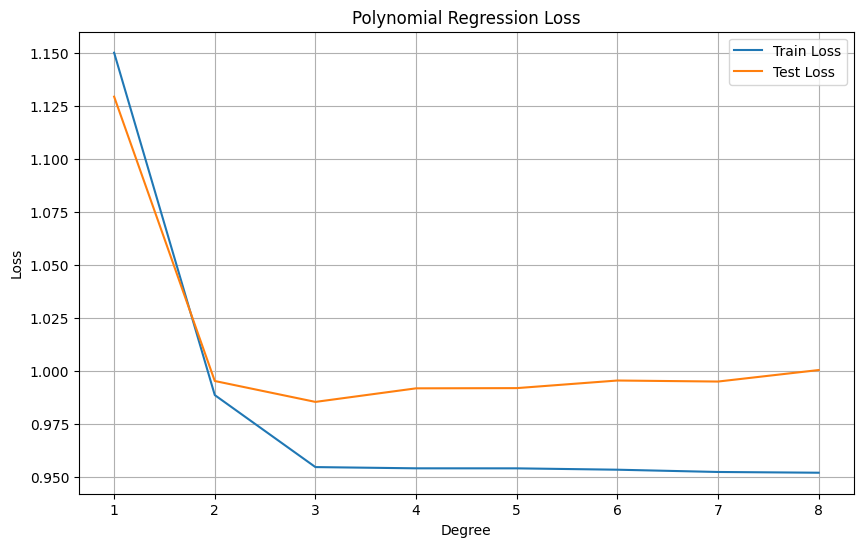
\includegraphics[width=\textwidth]{1_3.png}
  \caption{Plot of the Training and Test loss for a polynomial regression model}
\end{figure} 

It is evident that when the degree is low, both the train and test loss are decreasing. This is indicative of the model fitting the data well. However, as the degree increases, specifically the trend from degree = 4 to degree = 8, we start seeing the test loss start to increase. 
This is a sign of overfiting of the data as the model is fitting the training data too well and cannot generalize to new unseen samples. This behavior makes sense, as when our model capacity gets too great (high degree polynomial), the model will start to fit the noise in the data and not the underlying pattern. \\

\textbf{Question 1.4} \\
\begin{figure}[H]
  \centering
  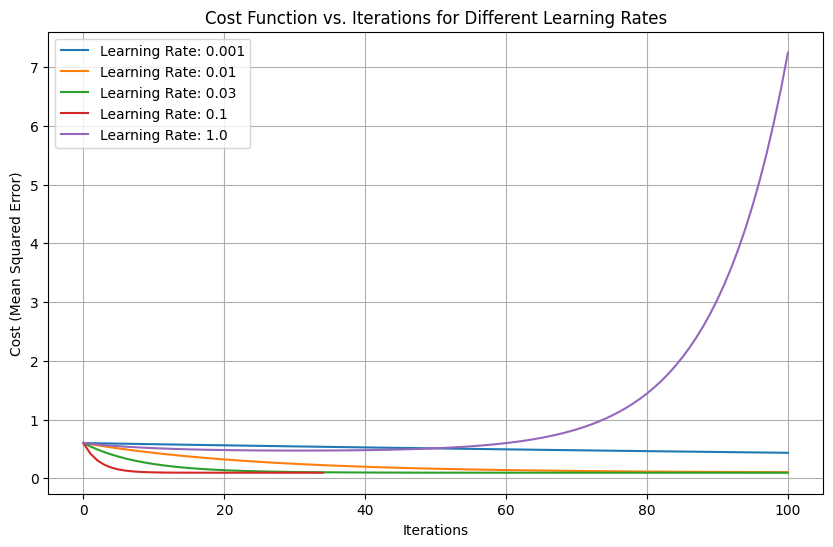
\includegraphics[width=\textwidth]{1_4.png}
  \caption{Training loss for different step sizes}
\end{figure} 


We can see that for the lower learning rates, the model converges to a lower loss than the initial loss. We notice too that the learning rates of 0.001 - 0.1. It is evident, however, that once we increase the learning rate too much, the loss 
no longer decreases and the model diverges. The massive increase for the learning rate of 1.0 is due to the fact that the model is overshooting the minimum and is unable to converge (gradient explodes). In our tests and based on the graph, it seems that learning rates 0.1, 0.03, and 0.01 are all approaching the same loss after 100 iterations and thus perform the best lowest loss. 


\end{document} 